\documentclass[twoside]{book}

% Packages required by doxygen
\usepackage{fixltx2e}
\usepackage{calc}
\usepackage{doxygen}
\usepackage[export]{adjustbox} % also loads graphicx
\usepackage{graphicx}
\usepackage[utf8]{inputenc}
\usepackage{makeidx}
\usepackage{multicol}
\usepackage{multirow}
\PassOptionsToPackage{warn}{textcomp}
\usepackage{textcomp}
\usepackage[nointegrals]{wasysym}
\usepackage[table]{xcolor}

% Font selection
\usepackage[T1]{fontenc}
\usepackage[scaled=.90]{helvet}
\usepackage{courier}
\usepackage{amssymb}
\usepackage{sectsty}
\renewcommand{\familydefault}{\sfdefault}
\allsectionsfont{%
  \fontseries{bc}\selectfont%
  \color{darkgray}%
}
\renewcommand{\DoxyLabelFont}{%
  \fontseries{bc}\selectfont%
  \color{darkgray}%
}
\newcommand{\+}{\discretionary{\mbox{\scriptsize$\hookleftarrow$}}{}{}}

% Page & text layout
\usepackage{geometry}
\geometry{%
  a4paper,%
  top=2.5cm,%
  bottom=2.5cm,%
  left=2.5cm,%
  right=2.5cm%
}
\tolerance=750
\hfuzz=15pt
\hbadness=750
\setlength{\emergencystretch}{15pt}
\setlength{\parindent}{0cm}
\setlength{\parskip}{3ex plus 2ex minus 2ex}
\makeatletter
\renewcommand{\paragraph}{%
  \@startsection{paragraph}{4}{0ex}{-1.0ex}{1.0ex}{%
    \normalfont\normalsize\bfseries\SS@parafont%
  }%
}
\renewcommand{\subparagraph}{%
  \@startsection{subparagraph}{5}{0ex}{-1.0ex}{1.0ex}{%
    \normalfont\normalsize\bfseries\SS@subparafont%
  }%
}
\makeatother

% Headers & footers
\usepackage{fancyhdr}
\pagestyle{fancyplain}
\fancyhead[LE]{\fancyplain{}{\bfseries\thepage}}
\fancyhead[CE]{\fancyplain{}{}}
\fancyhead[RE]{\fancyplain{}{\bfseries\leftmark}}
\fancyhead[LO]{\fancyplain{}{\bfseries\rightmark}}
\fancyhead[CO]{\fancyplain{}{}}
\fancyhead[RO]{\fancyplain{}{\bfseries\thepage}}
\fancyfoot[LE]{\fancyplain{}{}}
\fancyfoot[CE]{\fancyplain{}{}}
\fancyfoot[RE]{\fancyplain{}{\bfseries\scriptsize Generated by Doxygen }}
\fancyfoot[LO]{\fancyplain{}{\bfseries\scriptsize Generated by Doxygen }}
\fancyfoot[CO]{\fancyplain{}{}}
\fancyfoot[RO]{\fancyplain{}{}}
\renewcommand{\footrulewidth}{0.4pt}
\renewcommand{\chaptermark}[1]{%
  \markboth{#1}{}%
}
\renewcommand{\sectionmark}[1]{%
  \markright{\thesection\ #1}%
}

% Indices & bibliography
\usepackage{natbib}
\usepackage[titles]{tocloft}
\setcounter{tocdepth}{3}
\setcounter{secnumdepth}{5}
\makeindex

% Hyperlinks (required, but should be loaded last)
\usepackage{ifpdf}
\ifpdf
  \usepackage[pdftex,pagebackref=true]{hyperref}
\else
  \usepackage[ps2pdf,pagebackref=true]{hyperref}
\fi
\hypersetup{%
  colorlinks=true,%
  linkcolor=blue,%
  citecolor=blue,%
  unicode%
}

% Custom commands
\newcommand{\clearemptydoublepage}{%
  \newpage{\pagestyle{empty}\cleardoublepage}%
}

\usepackage{caption}
\captionsetup{labelsep=space,justification=centering,font={bf},singlelinecheck=off,skip=4pt,position=top}

%===== C O N T E N T S =====

\begin{document}

% Titlepage & ToC
\hypersetup{pageanchor=false,
             bookmarksnumbered=true,
             pdfencoding=unicode
            }
\pagenumbering{alph}
\begin{titlepage}
\vspace*{7cm}
\begin{center}%
{\Large Random Binary Tree Generator }\\
\vspace*{1cm}
{\large Generated by Doxygen 1.8.13}\\
\end{center}
\end{titlepage}
\clearemptydoublepage
\pagenumbering{roman}
\tableofcontents
\clearemptydoublepage
\pagenumbering{arabic}
\hypersetup{pageanchor=true}

%--- Begin generated contents ---
\chapter{Simple Random Binary Tree Generator}
\label{md_README}
\Hypertarget{md_README}
\href{https://travis-ci.org/saber-dragon/RandomBinaryTreeGenerator}{\tt }

This repo implements a very simple random binary tree generator. The major purpose of this repo is to produce some test cases for binary-\/tree related problems on leetcode.

\subsection*{Usage}

see \href{./example.cpp}{\tt \char`\"{}example.\+cpp\char`\"{}}

\subsection*{Sample Output}

\begin{quote}
By {\ttfamily Simple\+Print}\+: \end{quote}

\begin{DoxyCode}
\{val : 6724, left : 9480, right : 223\}
\{val : 9480, left : 3885, right : 300\}
\{val : 3885, left : 8074, right : 9900\}
\{val : 8074, left : 9191, right : NULL\}
\{val : 9191, left : NULL, right : NULL\}
\{val : 9900, left : NULL, right : NULL\}
\{val : 300, left : 7552, right : NULL\}
\{val : 7552, left : NULL, right : 3938\}
\{val : 3938, left : NULL, right : NULL\}
\{val : 223, left : NULL, right : NULL\}
\end{DoxyCode}


\begin{quote}
By {\ttfamily Tree\+To\+Dot}\+: \end{quote}



\begin{DoxyCode}
digraph BinaryTree \{
node [shape = record,height=.1];
 node0[label = "<f0> |<f1> 6724|<f2> "];
 node1[label = "<f0> |<f1> 9480|<f2> "];
 node2[label = "<f0> |<f1> 3885|<f2> "];
 node3[label = "<f0> |<f1> 8074|<f2> "];
 node4[label = "<f0> |<f1> 9191|<f2> "];
 node5[label = "<f0> |<f1> 9900|<f2> "];
 node6[label = "<f0> |<f1> 300|<f2> "];
 node7[label = "<f0> |<f1> 7552|<f2> "];
 node8[label = "<f0> |<f1> 3938|<f2> "];
 node9[label = "<f0> |<f1> 223|<f2> "];
"node0":f0 -> "node1":f1;
"node1":f0 -> "node2":f1;
"node2":f0 -> "node3":f1;
"node3":f0 -> "node4":f1;
"node2":f2 -> "node5":f1;
"node1":f2 -> "node6":f1;
"node6":f0 -> "node7":f1;
"node7":f2 -> "node8":f1;
"node0":f2 -> "node9":f1;
\}
\end{DoxyCode}
 Note that the dot file can be viewed visualized with {\ttfamily xdot} or you can use {\ttfamily graphviz} to get the P\+NG by simple running {\ttfamily dot -\/\+Tpng -\/o example.\+png bt.\+dot}. The resulted P\+NG is shown below.

 
\chapter{Class Index}
\section{Class List}
Here are the classes, structs, unions and interfaces with brief descriptions\+:\begin{DoxyCompactList}
\item\contentsline{section}{\hyperlink{structTreeNode}{Tree\+Node} \\*Class for tree node }{\pageref{structTreeNode}}{}
\item\contentsline{section}{\hyperlink{classTreeUtil}{Tree\+Util} \\*Tree utility class }{\pageref{classTreeUtil}}{}
\end{DoxyCompactList}

\chapter{Class Documentation}
\hypertarget{structTreeNode}{}\section{Tree\+Node Struct Reference}
\label{structTreeNode}\index{Tree\+Node@{Tree\+Node}}


Class for tree node.  




{\ttfamily \#include $<$random\+Binary\+Tree.\+hpp$>$}



Collaboration diagram for Tree\+Node\+:
\nopagebreak
\begin{figure}[H]
\begin{center}
\leavevmode
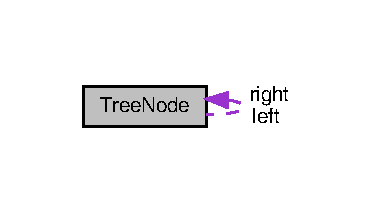
\includegraphics[width=179pt]{structTreeNode__coll__graph}
\end{center}
\end{figure}
\subsection*{Public Member Functions}
\begin{DoxyCompactItemize}
\item 
\mbox{\Hypertarget{structTreeNode_a984a98d5ccf7ef1f5a18094c6821f35d}\label{structTreeNode_a984a98d5ccf7ef1f5a18094c6821f35d}} 
\hyperlink{structTreeNode_a984a98d5ccf7ef1f5a18094c6821f35d}{Tree\+Node} ()
\begin{DoxyCompactList}\small\item\em Default constructor. \end{DoxyCompactList}\item 
\mbox{\Hypertarget{structTreeNode_a584fbc6fc6a5df73d9ab1603a5880cb0}\label{structTreeNode_a584fbc6fc6a5df73d9ab1603a5880cb0}} 
\hyperlink{structTreeNode_a584fbc6fc6a5df73d9ab1603a5880cb0}{Tree\+Node} (int val)
\begin{DoxyCompactList}\small\item\em Constructor specifies the val field. \end{DoxyCompactList}\end{DoxyCompactItemize}
\subsection*{Public Attributes}
\begin{DoxyCompactItemize}
\item 
\mbox{\Hypertarget{structTreeNode_a345b64c9d6ca399a45b516a1c7afd0eb}\label{structTreeNode_a345b64c9d6ca399a45b516a1c7afd0eb}} 
int {\bfseries val}
\item 
\mbox{\Hypertarget{structTreeNode_a5335e7d975822e87088ec2afdefb1736}\label{structTreeNode_a5335e7d975822e87088ec2afdefb1736}} 
\hyperlink{structTreeNode}{Tree\+Node} $\ast$ {\bfseries left}
\item 
\mbox{\Hypertarget{structTreeNode_a71b4faa364404d671943562b352b1b74}\label{structTreeNode_a71b4faa364404d671943562b352b1b74}} 
\hyperlink{structTreeNode}{Tree\+Node} $\ast$ {\bfseries right}
\end{DoxyCompactItemize}


\subsection{Detailed Description}
Class for tree node. 

The documentation for this struct was generated from the following file\+:\begin{DoxyCompactItemize}
\item 
random\+Binary\+Tree.\+hpp\end{DoxyCompactItemize}

\hypertarget{classTreeUtil}{}\section{Tree\+Util Class Reference}
\label{classTreeUtil}\index{Tree\+Util@{Tree\+Util}}


Tree utility class.  




{\ttfamily \#include $<$random\+Binary\+Tree.\+hpp$>$}



Collaboration diagram for Tree\+Util\+:
\nopagebreak
\begin{figure}[H]
\begin{center}
\leavevmode
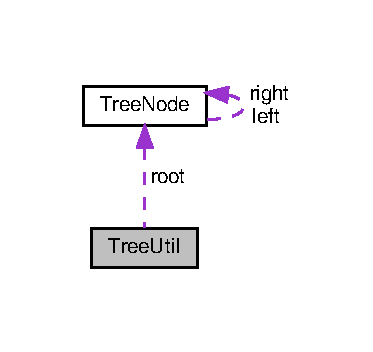
\includegraphics[width=179pt]{classTreeUtil__coll__graph}
\end{center}
\end{figure}
\subsection*{Public Member Functions}
\begin{DoxyCompactItemize}
\item 
\hyperlink{classTreeUtil_a5e1dfba5f1f3574c2cc73720d3569fe2}{Tree\+Util} (\hyperlink{structTreeNode}{Tree\+Node} $\ast$root)
\begin{DoxyCompactList}\small\item\em Constructor. \end{DoxyCompactList}\item 
void \hyperlink{classTreeUtil_ac7dffdfd7262dd5451b85c5089ece102}{Tree\+To\+Dot\+Edge} (std\+::ostream \&os, \hyperlink{structTreeNode}{Tree\+Node} $\ast$cur, size\+\_\+t my\+\_\+id)
\begin{DoxyCompactList}\small\item\em Tree edge to output stream in dot-\/format. \end{DoxyCompactList}\item 
void \hyperlink{classTreeUtil_aa39fa77d519ea3449e35fcaa73a2230b}{Tree\+To\+Dot\+Node} (std\+::ostream \&os, \hyperlink{structTreeNode}{Tree\+Node} $\ast$cur)
\begin{DoxyCompactList}\small\item\em Tree node to output stream in dot-\/format. \end{DoxyCompactList}\item 
void \hyperlink{classTreeUtil_a42bc4c25bf0e2aeb12ce35f3e0782ec3}{Tree\+To\+Dot} (std\+::ostream \&os)
\begin{DoxyCompactList}\small\item\em Tree to output stream in dot-\/format. \end{DoxyCompactList}\item 
void \hyperlink{classTreeUtil_af6d09d8d92320373731994e39549dd9e}{Simple\+Print} (std\+::ostream \&os)
\begin{DoxyCompactList}\small\item\em Simple print. \end{DoxyCompactList}\item 
void \hyperlink{classTreeUtil_a0d0a0988dc7036d1000afffcd3477866}{Simple\+Print\+Rec} (std\+::ostream \&os, \hyperlink{structTreeNode}{Tree\+Node} $\ast$cur)
\begin{DoxyCompactList}\small\item\em Simple print recursively. \end{DoxyCompactList}\item 
void \hyperlink{classTreeUtil_ab7617a40a2b508602c5094667c318a4f}{Inorder\+Print} (std\+::ostream \&os)
\begin{DoxyCompactList}\small\item\em Inorder print. \end{DoxyCompactList}\item 
\mbox{\Hypertarget{classTreeUtil_a0674a543776ed3c8de207f8e3d6a29a3}\label{classTreeUtil_a0674a543776ed3c8de207f8e3d6a29a3}} 
void \hyperlink{classTreeUtil_a0674a543776ed3c8de207f8e3d6a29a3}{Inorder\+Print\+Rec} (std\+::ostream \&os, \hyperlink{structTreeNode}{Tree\+Node} $\ast$cur)
\begin{DoxyCompactList}\small\item\em Inorder print recursively. \end{DoxyCompactList}\end{DoxyCompactItemize}
\subsection*{Public Attributes}
\begin{DoxyCompactItemize}
\item 
\mbox{\Hypertarget{classTreeUtil_abdfd330694b0f7f9d59a0400db7b05b4}\label{classTreeUtil_abdfd330694b0f7f9d59a0400db7b05b4}} 
\hyperlink{structTreeNode}{Tree\+Node} $\ast$ {\bfseries root}
\item 
size\+\_\+t \hyperlink{classTreeUtil_a9b39a7cbe992826ad451627f87277804}{id}
\end{DoxyCompactItemize}


\subsection{Detailed Description}
Tree utility class. 

This class provides many useful A\+P\+Is which can be applied to a tree. 

\subsection{Constructor \& Destructor Documentation}
\mbox{\Hypertarget{classTreeUtil_a5e1dfba5f1f3574c2cc73720d3569fe2}\label{classTreeUtil_a5e1dfba5f1f3574c2cc73720d3569fe2}} 
\index{Tree\+Util@{Tree\+Util}!Tree\+Util@{Tree\+Util}}
\index{Tree\+Util@{Tree\+Util}!Tree\+Util@{Tree\+Util}}
\subsubsection{\texorpdfstring{Tree\+Util()}{TreeUtil()}}
{\footnotesize\ttfamily Tree\+Util\+::\+Tree\+Util (\begin{DoxyParamCaption}\item[{\hyperlink{structTreeNode}{Tree\+Node} $\ast$}]{root }\end{DoxyParamCaption})\hspace{0.3cm}{\ttfamily [inline]}, {\ttfamily [explicit]}}



Constructor. 

global id 

\subsection{Member Function Documentation}
\mbox{\Hypertarget{classTreeUtil_ab7617a40a2b508602c5094667c318a4f}\label{classTreeUtil_ab7617a40a2b508602c5094667c318a4f}} 
\index{Tree\+Util@{Tree\+Util}!Inorder\+Print@{Inorder\+Print}}
\index{Inorder\+Print@{Inorder\+Print}!Tree\+Util@{Tree\+Util}}
\subsubsection{\texorpdfstring{Inorder\+Print()}{InorderPrint()}}
{\footnotesize\ttfamily void Tree\+Util\+::\+Inorder\+Print (\begin{DoxyParamCaption}\item[{std\+::ostream \&}]{os }\end{DoxyParamCaption})\hspace{0.3cm}{\ttfamily [inline]}}



Inorder print. 

Similar as Simple\+Print\char`\"{}()\char`\"{}, but print the tree in an inorder manner.


\begin{DoxyParams}{Parameters}
{\em os} & output stream \\
\hline
\end{DoxyParams}
\mbox{\Hypertarget{classTreeUtil_af6d09d8d92320373731994e39549dd9e}\label{classTreeUtil_af6d09d8d92320373731994e39549dd9e}} 
\index{Tree\+Util@{Tree\+Util}!Simple\+Print@{Simple\+Print}}
\index{Simple\+Print@{Simple\+Print}!Tree\+Util@{Tree\+Util}}
\subsubsection{\texorpdfstring{Simple\+Print()}{SimplePrint()}}
{\footnotesize\ttfamily void Tree\+Util\+::\+Simple\+Print (\begin{DoxyParamCaption}\item[{std\+::ostream \&}]{os }\end{DoxyParamCaption})\hspace{0.3cm}{\ttfamily [inline]}}



Simple print. 

This function simply print all nodes of the tree in the format\+: \{val \+: cur-\/$>$val, left \+: cur-\/$>$left-\/$>$val, right \+: cur-\/$>$right-\/$>$val\}. Note that if left/right does not exists, a string of \char`\"{}\+N\+U\+L\+L\char`\"{} will be used..


\begin{DoxyParams}{Parameters}
{\em os} & output stream \\
\hline
\end{DoxyParams}
\mbox{\Hypertarget{classTreeUtil_a0d0a0988dc7036d1000afffcd3477866}\label{classTreeUtil_a0d0a0988dc7036d1000afffcd3477866}} 
\index{Tree\+Util@{Tree\+Util}!Simple\+Print\+Rec@{Simple\+Print\+Rec}}
\index{Simple\+Print\+Rec@{Simple\+Print\+Rec}!Tree\+Util@{Tree\+Util}}
\subsubsection{\texorpdfstring{Simple\+Print\+Rec()}{SimplePrintRec()}}
{\footnotesize\ttfamily void Tree\+Util\+::\+Simple\+Print\+Rec (\begin{DoxyParamCaption}\item[{std\+::ostream \&}]{os,  }\item[{\hyperlink{structTreeNode}{Tree\+Node} $\ast$}]{cur }\end{DoxyParamCaption})\hspace{0.3cm}{\ttfamily [inline]}}



Simple print recursively. 

This function simply print all nodes of the tree rooted in cur.


\begin{DoxyParams}{Parameters}
{\em os} & output stream \\
\hline
{\em cur} & current node \\
\hline
\end{DoxyParams}
\mbox{\Hypertarget{classTreeUtil_a42bc4c25bf0e2aeb12ce35f3e0782ec3}\label{classTreeUtil_a42bc4c25bf0e2aeb12ce35f3e0782ec3}} 
\index{Tree\+Util@{Tree\+Util}!Tree\+To\+Dot@{Tree\+To\+Dot}}
\index{Tree\+To\+Dot@{Tree\+To\+Dot}!Tree\+Util@{Tree\+Util}}
\subsubsection{\texorpdfstring{Tree\+To\+Dot()}{TreeToDot()}}
{\footnotesize\ttfamily void Tree\+Util\+::\+Tree\+To\+Dot (\begin{DoxyParamCaption}\item[{std\+::ostream \&}]{os }\end{DoxyParamCaption})\hspace{0.3cm}{\ttfamily [inline]}}



Tree to output stream in dot-\/format. 

This function writes the tree into an output stream.


\begin{DoxyParams}{Parameters}
{\em os} & output stream \\
\hline
\end{DoxyParams}
\mbox{\Hypertarget{classTreeUtil_ac7dffdfd7262dd5451b85c5089ece102}\label{classTreeUtil_ac7dffdfd7262dd5451b85c5089ece102}} 
\index{Tree\+Util@{Tree\+Util}!Tree\+To\+Dot\+Edge@{Tree\+To\+Dot\+Edge}}
\index{Tree\+To\+Dot\+Edge@{Tree\+To\+Dot\+Edge}!Tree\+Util@{Tree\+Util}}
\subsubsection{\texorpdfstring{Tree\+To\+Dot\+Edge()}{TreeToDotEdge()}}
{\footnotesize\ttfamily void Tree\+Util\+::\+Tree\+To\+Dot\+Edge (\begin{DoxyParamCaption}\item[{std\+::ostream \&}]{os,  }\item[{\hyperlink{structTreeNode}{Tree\+Node} $\ast$}]{cur,  }\item[{size\+\_\+t}]{my\+\_\+id }\end{DoxyParamCaption})\hspace{0.3cm}{\ttfamily [inline]}}



Tree edge to output stream in dot-\/format. 

This function writes edges of the tree into an output stream.


\begin{DoxyParams}{Parameters}
{\em os} & output stream \\
\hline
{\em cur} & current node \\
\hline
{\em my\+\_\+id} & id of current node \\
\hline
\end{DoxyParams}
\mbox{\Hypertarget{classTreeUtil_aa39fa77d519ea3449e35fcaa73a2230b}\label{classTreeUtil_aa39fa77d519ea3449e35fcaa73a2230b}} 
\index{Tree\+Util@{Tree\+Util}!Tree\+To\+Dot\+Node@{Tree\+To\+Dot\+Node}}
\index{Tree\+To\+Dot\+Node@{Tree\+To\+Dot\+Node}!Tree\+Util@{Tree\+Util}}
\subsubsection{\texorpdfstring{Tree\+To\+Dot\+Node()}{TreeToDotNode()}}
{\footnotesize\ttfamily void Tree\+Util\+::\+Tree\+To\+Dot\+Node (\begin{DoxyParamCaption}\item[{std\+::ostream \&}]{os,  }\item[{\hyperlink{structTreeNode}{Tree\+Node} $\ast$}]{cur }\end{DoxyParamCaption})\hspace{0.3cm}{\ttfamily [inline]}}



Tree node to output stream in dot-\/format. 

This function writes nodes of the tree into an output stream.


\begin{DoxyParams}{Parameters}
{\em os} & output stream \\
\hline
{\em cur} & current node \\
\hline
\end{DoxyParams}


\subsection{Member Data Documentation}
\mbox{\Hypertarget{classTreeUtil_a9b39a7cbe992826ad451627f87277804}\label{classTreeUtil_a9b39a7cbe992826ad451627f87277804}} 
\index{Tree\+Util@{Tree\+Util}!id@{id}}
\index{id@{id}!Tree\+Util@{Tree\+Util}}
\subsubsection{\texorpdfstring{id}{id}}
{\footnotesize\ttfamily size\+\_\+t Tree\+Util\+::id}

tree root 

The documentation for this class was generated from the following file\+:\begin{DoxyCompactItemize}
\item 
random\+Binary\+Tree.\+hpp\end{DoxyCompactItemize}

%--- End generated contents ---

% Index
\backmatter
\newpage
\phantomsection
\clearemptydoublepage
\addcontentsline{toc}{chapter}{Index}
\printindex

\end{document}
